\chapter{Configuring and Building ITK}
\label{chapter:Installation}

This chapter describes the process for configuring and compiling ITK on your
system. Keep in mind that ITK is a toolkit, and as such, once it is installed
on your computer it does not provide an application to run. What ITK does
provide is a large set of libraries which can be used to create your own
applications. Besides the toolkit proper, ITK also includes an extensive set of
examples and tests that introduce ITK concepts and show how to use ITK in your
own projects.

Some of the examples distributed with ITK depend on third party libraries, some
of which may need to be installed separately. For the initial build of ITK, you
may want to ignore these extra libraries and just compile the toolkit itself.

ITK has been developed and tested across different combinations of operating
systems, compilers, and hardware platforms including Microsoft Windows, Linux on
various architectures, Solaris/UNIX, macOS, and Cygwin. Kitware is committed
to support the following compilers for building ITK:

% List updated according to information provided here:
% https://www.itk.org/Wiki/ITK_Release_4/Modern_C++#Fully_Committed_to_Support

\begin{itemize}
\item GCC 4.x
\item Visual Studio 8 SP 1 (until 2015), 9 (until 2018), 10 (until 2020)
\item Intel Compiler Suite 11.x, 12.x (including macOS release)
\item Darwin-c++-4.2 PPC (until 2015), x86\_64
\item Win32-mingw-gcc-4.5
\item Clang 3.3 and later
\end{itemize}

If you are currently using an outdated compiler this may be an excellent excuse
for upgrading this old piece of software! Support for different platforms is
evident on the ITK quality dashboard (see Section \ref{sec:CDash} on page
\pageref{sec:CDash}).

\section{Obtaining the Software}
\label{sec:ObtainingTheSoftware}
\label{sec:DownloadingITK}
\index{Downloading}

There are two different ways to access the ITK source code:
\begin{description}
  \item[Periodic releases]{Official releases are available on the ITK web
    site\footnote{\url{https://itk.org/ITK/resources/software.html}}.
    They are released twice a year,
    and announced on the ITK web pages and mailing list.
    However, they may not provide the latest and greatest features of the
    toolkit.}
  \item[Continuous repository checkout]{Direct access to the Git source code
    repository\footnote{\url{https://itk.org/ITK.git}} provides immediate
    availability to the latest toolkit additions. But, on any given day the
    source code may not be stable as compared to the official releases.}
\end{description}

This software guide assumes that you are using the current released version of
ITK, available on the ITK web site. If you are a new user, we recommend the
released version of the software. It is more consistent
than the code available from the Git repository (see Section
\ref{sec:DownloadingFromGit}).  When working from the
repository, please be aware of the ITK quality testing dashboard. The Insight
Toolkit is heavily tested using the open-source CDash regression testing
system\footnote{\url{http://open.cdash.org/index.php?project=Insight}}. Before
updating the repository, make sure that the dashboard is \emph{green},
indicating stable code. (Learn more about the ITK dashboard and quality
assurance process in Section \ref{sec:CDash} on page \pageref{sec:CDash}.)

\subsection{Downloading Packaged Releases}
\label{sec:DownloadingReleases}

\index{ITK!downloading release}

ITK can be downloaded without cost from the following web site:
\begin{center}
  \url{https://www.itk.org/ITK/resources/software.html}
\end{center}

On the web page, choose the tarball that better fits your system. The options are
\code{.zip} and \code{.tar.gz} files. The first type is better suited for
Microsoft-Windows, while the second one is the preferred format for UNIX
systems.

Once you unzip or untar the file a directory called
\code{InsightToolkit-\ITKVERSIONMAJORMINORPATCH} will be created in your disk and
you will be ready to start the configuration process described in Section
\ref{sec:CMakeforITK} on page \pageref{sec:CMakeforITK}.

\subsection{Downloading From Git}
\label{sec:DownloadingFromGit}

\index{ITK!Git repository}

Git is a free and open source distributed version control system.  For more
information about Git please see Section \ref{sec:GitRepository} on page
\pageref{sec:GitRepository}. (Note: please make sure that you access the
software via Git only when the ITK quality dashboard indicates that the code
is stable.)

Access ITK via Git using the following commands (under a Git Bash shell):
\begin{minted}[baselinestretch=1,fontsize=\footnotesize,linenos=false,bgcolor=ltgray]{bash}
git clone git://itk.org/ITK.git
\end{minted}

This will trigger the download of the software into a directory named
\code{ITK}.  Any time you want to update your version, it will be enough to
change into this directory, \code{ITK}, and type:
\begin{minted}[baselinestretch=1,fontsize=\footnotesize,linenos=false,bgcolor=ltgray]{cpp}
git pull
\end{minted}

Once you obtain the software you are ready to configure and compile it (see
Section \ref{sec:CMakeforITK} on page \pageref{sec:CMakeforITK}). First,
however, we recommend reading the following sections that describe the
organization of the software and joining the mailing list.

\subsection{Data}
\label{sec:Data}

The Insight Toolkit was designed to support the Visible Human Project
and its associated data. This data is available from the National Library of
Medicine at \url{http://www.nlm.nih.gov/research/visible/visible_human.html}.

Another source of data can be obtained from the ITK Web site at either
of the following:
\begin{quote}
\url{https://www.itk.org/ITK/resources/links.html} \\
\url{ftp://public.kitware.com/pub/itk/Data/}.
\end{quote}

\section{Using CMake for Configuring and Building ITK}
\label{sec:UsingCMakeForConfiguringAndBuildingITK}

The challenge of supporting ITK across platforms has been solved through the
use of CMake\footnote{\url{www.cmake.org}}, a cross-platform, open-source build
system. CMake controls the software compilation process with simple platform
and compiler-independent configuration files. CMake is quite sophisticated---it
supports complex environments requiring system introspection, compiler feature
testing, and code generation.

CMake generates native Makefiles or workspaces to be used with the corresponding
development environment of your choice. For example, on UNIX and Cygwin systems,
CMake generates Makefiles; under Microsoft Windows CMake generates Visual Studio
workspaces; CMake is also capable of generating appropriate build files for
other development environments, e.g., Eclipse. The information used by CMake is
provided in \code{CMakeLists.txt} files that are present in every directory of
the ITK source tree. Along with the specification of project structure and code
dependencies these files specify the information that need to be provided to
CMake by the user during project configuration stage. Typical configuration
options specified by the user include paths to utilities installed on your
system and selection of software features to be included.

An ITK build requires only CMake and a C++ compiler. ITK ships with all the
third party library dependencies required, and these dependencies are used
during compilation unless the use of a system version is requested during CMake
configuration.

\subsection{Preparing CMake}
\label{sec:CMakeforITK}

\index{CMake}
\index{CMake!downloading}

CMake can be downloaded at no cost from
\begin{center}
  \url{https://cmake.org/download/}
\end{center}

You can download binary versions for most of the popular platforms including
Microsoft Windows, macOS, Linux, PowerPC and IRIX. Alternatively you can
download the source code and build CMake on your system. Follow the instructions
provided on the CMake web page for downloading and installing the software. The
minimum version of CMake has been evolving along with the version of ITK. For
example, the current version of ITK (\ITKVERSIONMAJORMINORPATCH) requires the minimum
CMake version to be 2.8.9.

CMake provides a terminal-based interface (Figure \ref{fig:CMakeGUI})
on platforms support the \code{curses} library. For most platforms CMake also
provides a GUI based on the Qt library. Figure \ref{fig:CMakeGUI} shows the
terminal-based CMake interface for Linux and CMake GUI for Microsoft Windows.

\begin{figure}[htb!]
\centering
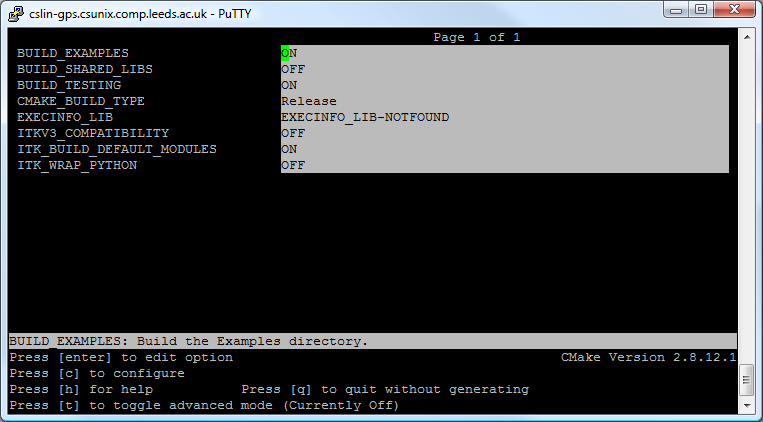
\includegraphics[width=0.8\textwidth]{ccmake-2-8-screenshot.eps}
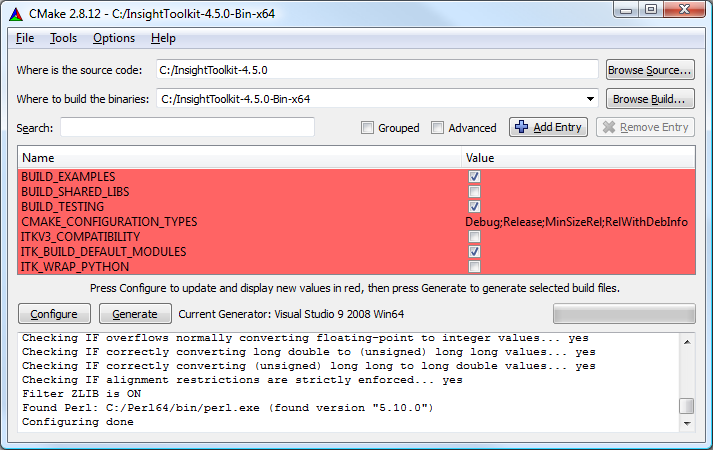
\includegraphics[width=0.8\textwidth]{cmake-gui-2-8-win-screenshot.eps}
\itkcaption[CMake user interface]{CMake user interfaces: at the top is the
interface based on the \code{curses} library supported by UNIX/Linux systems,
below is the Microsoft Windows version of the CMake GUI based on the Qt library
(CMake GUI is also available on UNIX/Linux systems).}
\label{fig:CMakeGUI}
\end{figure}

Running CMake to configure and prepare for compilation a new project initially
requires two pieces of information: where the source code directory is located,
and where the compiled code is to be produced. These are referred to as the
\emph{source directory} and the \emph{binary directory} respectively.
We recommend setting the binary directory to be different than the source
directory in order to produce an \emph{out-of-source} build.

If you choose to use the terminal-based version of CMake (\code{ccmake}) the
binary directory needs to be created first and then CMake is invoked from the
binary directory with the path to the source directory. For example:

\small
\begin{minted}[baselinestretch=1,fontsize=\footnotesize,linenos=false,bgcolor=ltgray]{bash}
mkdir ITK-build
cd ITK-build
ccmake ../ITK
\end{minted}
\normalsize

In the GUI version of CMake (\code{cmake-gui}) the source and binary directories
are specified in the appropriate input fields (Figure \ref{fig:CMakeGUI}) and
the application will request a confirmation to create a new binary directory if
it does not exist.

CMake runs in an interactive mode which allows iterative selection of options
followed by configuration according to the updated options. This iterative
process proceeds until no more options remain to be specified. At this point, a
generation step produces the appropriate build files for your configuration.

This interactive configuration process can be better understood by imagining
the traversal of a path in a decision tree. Every selected option introduces the
possibility that new, dependent options may become relevant. These new options
are presented by CMake at the top of the options list in its interface. Only
when no new options appear after a configuration iteration can you be sure that
the necessary decisions have all been made. At this point build files are
generated for the current configuration.

\subsection{Configuring ITK}
\label{sec:ConfigureITK}

\index{ITK!configuration}

Start terminal-based CMake interface \code{ccmake} on Linux and UNIX, or the
graphical user interface \code{cmake-gui} on Microsoft Windows. Remember to run
\code{ccmake} from the binary directory on Linux and UNIX. On Windows, specify
the source and binary directories in the GUI, then set and modify the
configuration and build option in the interface as necessary.

The examples distributed with the toolkit provide a helpful resource for
learning how to use ITK components but are not essential for compiling the
toolkit itself. The testing section of the source tree includes a large number
of small programs that exercise the capabilities of ITK classes. Enabling the
compilation of the examples and unit tests will considerably increase the build
time. In order to speed up the build process, you can disable the compilation of
the unit tests and examples. This is done by setting the variables
\code{BUILD\_TESTING} and \code{BUILD\_EXAMPLES} to \code{OFF}.

Most CMake variables in ITK have sensible default values. Each time a CMake
variable is changed, it is necessary to re-run the configuration step. In the
terminal-based version of the interface the configuration step is triggered by
hitting the ``c'' key. In the GUI version this is done by clicking on the
``Configure'' button.

When no new options appear highlighted in CMake, you can proceed to generate
Makefiles, a Visual Studio workspace, or other appropriate build files depending
on your preferred development environment. This is done in the GUI interface by
clicking on the ``Generate'' button. In the terminal-based version this is done
by hitting the ``g'' key. After the generation process the terminal-based
version of CMake will quit silently. The GUI window of CMake can be left open
for further refinement of configuration options as described in the next
section. With this scenario it is important to generate new build files to
reflect the latest configuration changes. In addition, the new build files need
to be reloaded if the project is open in the integrated development environment
such as Visual Studio or Eclipse.

\subsection{Advanced Module Configuration}
\label{sec:ModuleConfiguration}

\index{ITK!advanced configuration}
\index{ITK!modules}

Following the default configuration introduced in \ref{sec:ConfigureITK},
the majority of the toolkit will be built. The modern modular structure of the
toolkit makes it possible to customize the ITK library by choosing which modules
to include in the build. ITK was officially modularized in version 4.0.0
released in December of 2011. Developers have been testing and improving the
modular structure since then. The toolkit currently contains more than 100
regular/internal modules and many remote modules, while new ITK modules are
being developed.

\code{ITK\_BUILD\_DEFAULT\_MODULES} is the CMake option to build all default
modules in the toolkit, by default this option is \code{ON} as shown in Figure
\ref{fig:CMakeGUI}. The default modules include most internal ITK modules except
the ones that depend on external third party libraries (such as
\code{ITKVtkGlue}, \code{ITKBridgeOpenCV}, \code{ITKBridgeVXL}, etc.) and
several modules containing legacy code (\code{ITKReview}, \code{ITKDeprecated}
and \code{ITKv3Compatibility}).

Apart from the default mode of selecting the modules for building the ITK
library there are two other approaches module selection: the group mode, and the
advanced module mode. When \code{ITK\_BUILD\_DEFAULT\_MODULES} is set to
\code{OFF}, the selection of modules to be included in the ITK library can be
customized by changing the variables enabling group and advanced module
selection.

\code{ITKGroup\_\{group name\}} variables for group module selection are visible
when \code{ITK\_BUILD\_DEFAULT\_MODULES} is \code{OFF}. The ITK source code tree
is organized in such way that a group of modules characterised by close
relationships or similar functionalities stay in one subdirectory. Currently
there are 11 groups (excluding the External and Remote groups). The CMake
\code{ITKGroup\_\{group name\}} options are created for the convenient enabling
or disabling of multiple modules at once. The \code{ITKGroup\_Core} group is
selected by default as shown in Figure \ref{fig:ConfigITKGroup}. When a group is
selected, all modules in the group and their depending modules are enabled. When
a group variable is set to \code{OFF}, all modules in the group, except the ones
that are required by other enabled modules, are disabled.

\begin{figure}[htb!]
\centering
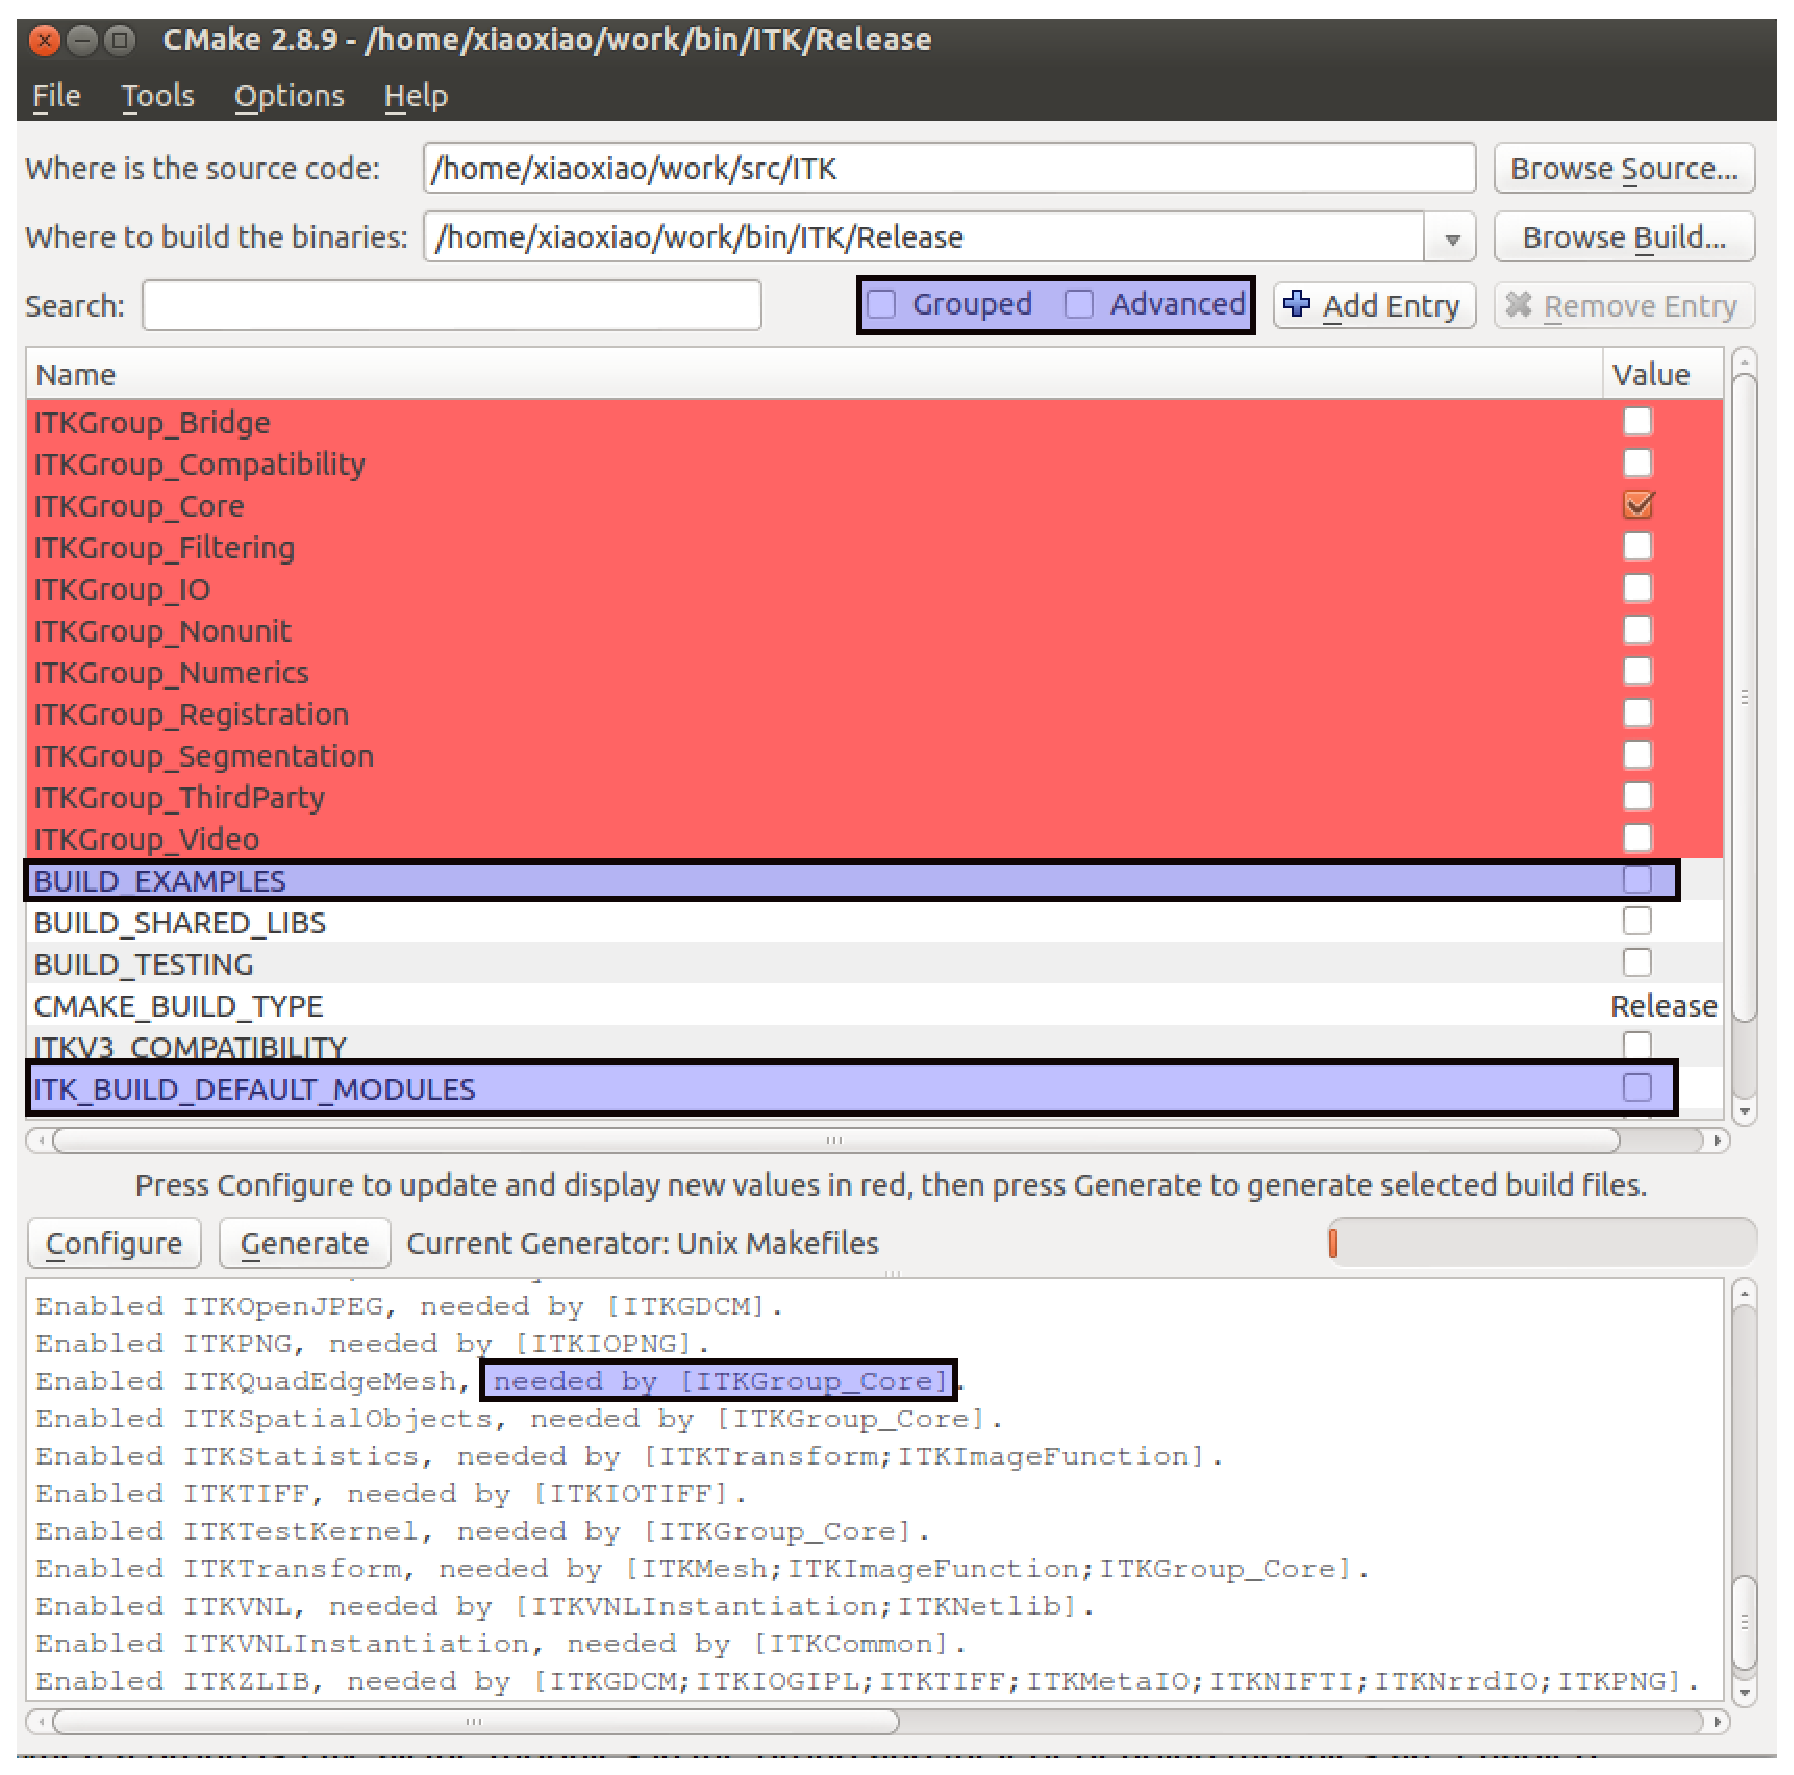
\includegraphics[width=0.8\textwidth]{Configure_ITK_Group.eps}
\itkcaption[ITK Group Configuration]{CMake GUI shows the ITK Group options.}
\label{fig:ConfigITKGroup}
\end{figure}

If you are not sure about which groups to turn on, but you do have a list of
specific modules to be included in your ITK library, you can certainly skip the
Group options and use the \code{Module\_\{module name\}} options only. Whatever
modules you select, their dependent modules are automatically enabled. In the
advanced mode of the CMake GUI, you can manually toggle the build of the
non-default modules via the \code{Module\_\{module name\}} variables. In Figure
\ref{fig:ConfigITKDefault} all default modules' \code{Module\_\{module name\}}
variables are shown disabled for toggling since they are enabled via the
\code{ITK\_BUILD\_DEFAULT\_MODULES} set to \code{ON} variable.

\begin{figure}[htb!]
\centering
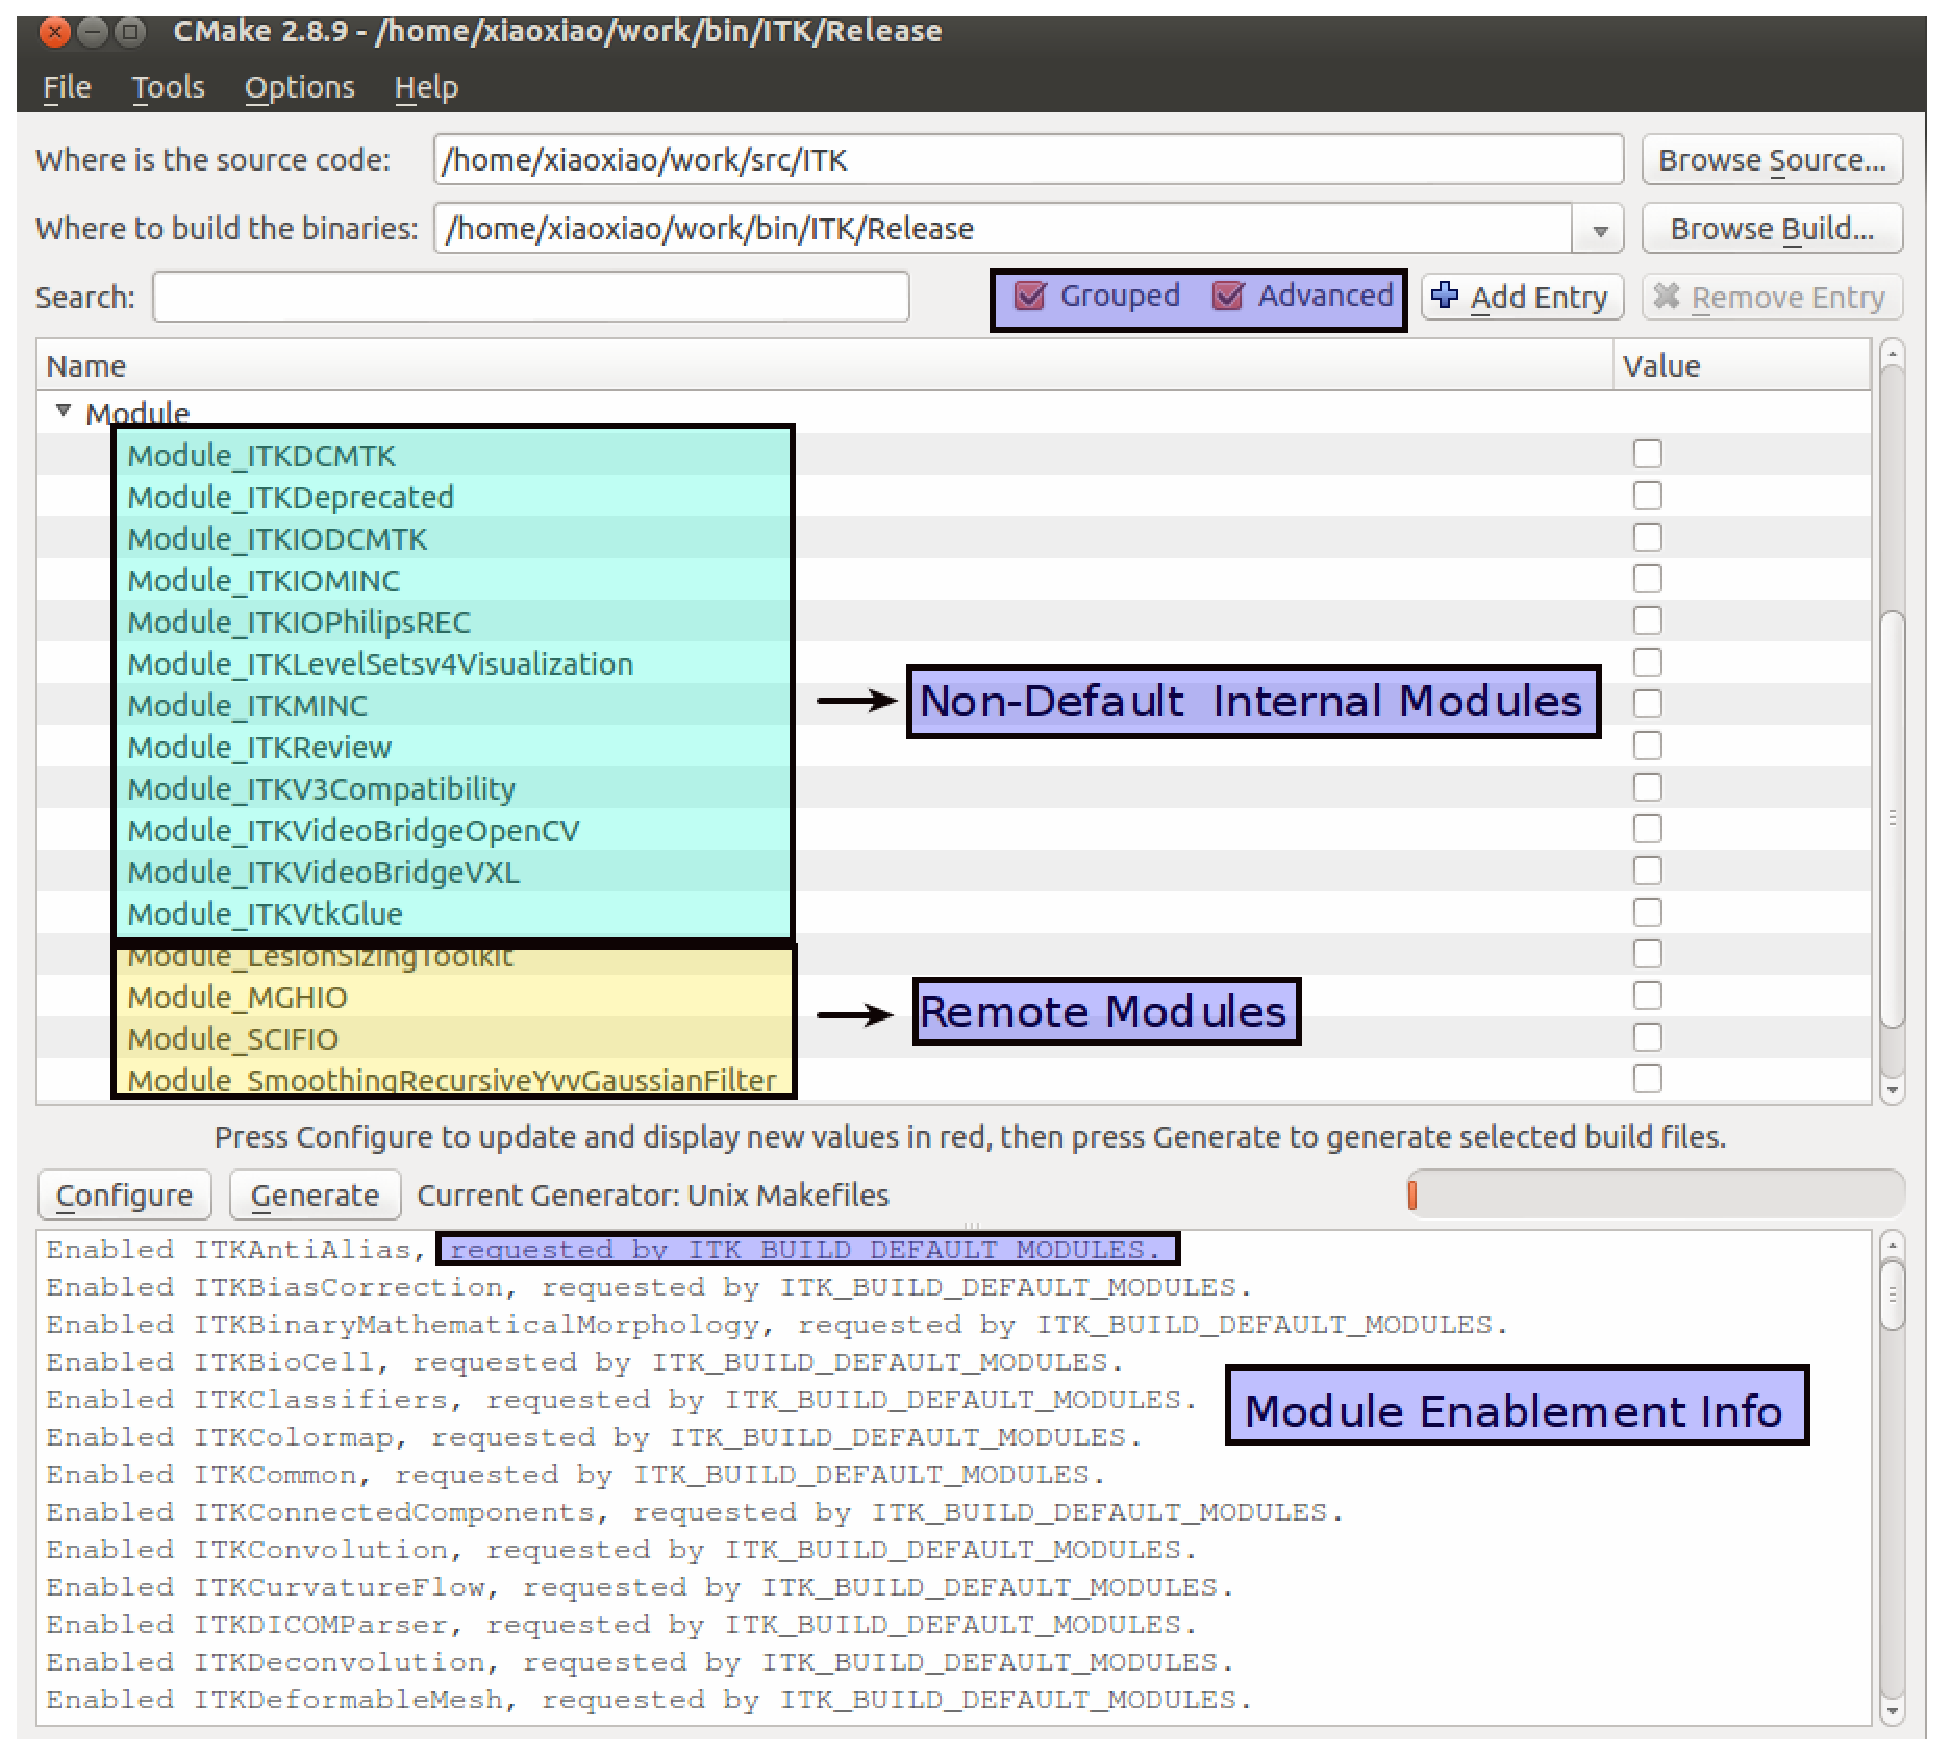
\includegraphics[width=0.8\textwidth]{Configure_ITK_Default.eps}
\itkcaption[Default ITK Configuration]{CMake GUI for configuring ITK: the
advanced mode shows options for non-default ITK Modules.}
\label{fig:ConfigITKDefault}
\end{figure}

However, not all modules will be visible in the CMake GUI at all times due to
the various levels of controls in the previous two modes. If some modules are
already enabled by other modes, these modules are set as internal variables and
are hidden in the CMake GUI. For example, \code{Module\_ITKFoo} variable is
hidden when the module \code{ITKFoo} is enabled in either of the following
scenarios:
\begin{enumerate}
\item module \code{ITKBar} is enabled and depends on \code{ITKFoo},
\item \code{ITKFoo} belongs to the group \code{ITKGroup\_FooAndBar} and the
group is enabled
\item \code{ITK\_BUILD\_DEFAULT\_MODULES} is \code{ON} and \code{ITKFoo} is a
default module.
\end{enumerate}

To find out why a particular module is enabled, check the CMake configuration
messages where the information about enabling or disabling the modules is
displayed (Figure \ref{fig:ConfigITKDefault}); these messages are sorted in
alphabetical order by module names.


\subsection{Static and Shared Libraries}
\label{sec:StaticSharedLibraries}

ITK libraries can be built as \textit{static libraries}, i.e. files whose
functions and variables are included in a binary during the link phase of
the build cycle. Alternatively, ITK libraries can be built as
\textit{shared libraries}, where libraries are dynamically linked to a
binary. In this case, functions and variables are shared at runtime according
to their symbols.

By enabling the standard CMake configuration variable,
\code{BUILD\_SHARED\_LIBS}, ITK modules with the \code{ENABLE\_SHARED} option
(see Section~\ref{sec:NameAndDependencies}) will be built as shared libraries.

Static libraries are preferred when creating a stand-alone executable. An
application can be distributed as a single file when statically linked.
Additional effort is not required to package library dependencies, configure the
system to find library dependencies at runtime, or define symbol export
specifications.

Shared libraries should be used when ITK is linked to more than one binary in
an application. This reduces binary size and ensures that singleton
variables are unique across the application.

A very advanced CMake configuration variable,
\code{ITK\_TEMPLATE\_VISIBILITY\_DEFAULT} defines the symbol visibility
attribute on template classes to \textit{default} on systems that require it
to perform \code{dynamic\_cast}'s on pointers passed across binaries. The
default value can be disabled only when it is known that template classes are
not implicitly instantiated and passed across binaries.


\subsection{Compiling ITK}
\label{sec:BuildITK}

\index{ITK!building}

To initiate the build process after generating the build files on Linux or UNIX,
simply type \code{make} in the terminal if the current directory is set to the
ITK binary directory. If using Visual Studio, first load the workspace named
\code{ITK.sln} from the binary directory specified in the CMake GUI and then
start the build by selecting ``Build Solution'' from the ``Build'' menu
or right-clicking on the \code{ALL\_BUILD} target in the Solution Explorer pane
and selecting the ``Build'' context menu item.

The build process can take anywhere from 15 minutes to a couple of hours,
depending on the the build configuration and the performance of your
system. If testing is enabled as part of the normal build process,
about 2400 test programs will be compiled. In this case, you will then need
to run \code{ctest} to verify that all the components of ITK have been correctly built
on your system.

\subsection{Installing ITK on Your System}
\label{sec:Installation}

\index{ITK!installation}

When the build process is complete an ITK binary distribution package can be
generated for installation on your system or on a system with compatible
specifications (such as hardware platform and operating system) as well as
suitable development environment components (such as C++ compiler and CMake).
The default prefix for installation destination directory needs to be specified
during CMake configuration process prior to compiling ITK. The installation
destination prefix can to be set through the CMake cache variable
\code{CMAKE\_INSTALL\_PREFIX}.

Typically distribution packages are generated to provide a ``clean'' form of the
software which is isolated from the details of the build process (separate from
the source and build trees). Due to the intended use of ITK as a toolkit for
software development the step of generating ITK binary packages for installing
ITK on other systems has limited application and thus it can be treated as
optional. However, the step for generating binary distribution packages has a
much wide application for distributing software developed with ITK. Further
details on configuring and generating binary packages with CMake can be found in
the CMake tutorial\footnote{\url{https://cmake.org/cmake-tutorial/}}.

\section{Getting Started With ITK}
\label{sec:GettingStartedWithITK}

The simplest way to create a new project with ITK is to create two new
directories somewhere in your disk, one to hold the source code and one to
hold the binaries and other files that are created in the build process. For
this example, create a \code{HelloWorldITK} directory to hold the source and a
\code{HelloWorldITK-build} directory to hold the binaries. The first file to
place in the source directory is a \code{CMakeLists.txt} file that will be
used by CMake to generate a Makefile (if you are using Linux or UNIX) or a
Visual Studio workspace (if you are using Microsoft Windows). The second source
file to be created is an actual C++ program that will exercise some of the large
number of classes available in ITK. The details of these files are described in
the following section.

Once both files are in your directory you can run CMake in order to configure
your project. Under UNIX/Linux, you can \code{cd} to your newly created binary
directory and launch the terminal-based version of CMake by entering
``\code{ccmake ../HelloWorldITK}'' in the terminal. Note the
``../HelloWorldITK'' in the command line to indicate that the
\code{CMakeLists.txt} file is up one directory and in \code{HelloWorldITK}.
In CMake GUI which can be used under Microsoft Windows and UNIX/Linux, the
source and binary directories will have to be specified prior to the
configuration and build file generation process.

Both the terminal-based and GUI versions of CMake will require you to specify
the directory where ITK was built in the CMake variable \code{ITK\_DIR}. The ITK
binary directory will contain a file named \code{ITKConfig.cmake} generated
during ITK configuration process with CMake. From this file, CMake will recover
all information required to configure your new ITK project.

After generating the build files, on UNIX/Linux systems the project can be
compiled by typing \code{make} in the terminal provided the current directory
is set to the project's binary directory. In Visual Studio on Microsoft Windows
the project can be built by loading the workspace named \code{HelloWorldITK.sln}
from the binary directory specified in the CMake GUI and selecting
``Build Solution'' from the ``Build'' menu or by right-clicking on
the \code{ALL\_BUILD} target in the Solution Explorer pane and selecting
the ``Build'' context menu item.

The resulting executable, which will be called \code{HelloWorld}, can be
executed on the command line. If on Microsoft Windows, please note that
double-clicking on the icon of the executable will quickly launch a command line
window, run the executable and close the window right away, not giving you time
to see the output. It is therefore preferable to run the executable from the DOS
command line by starting the \code{cmd.exe} shell first.

\subsection{Hello World!}
\label{sec:HelloWorldITK}

\index{Hello World}

This section provides and explains the contents of the two files which need to
be created for your new project. These two files can be found in the
\code{ITK/Examples/Installation} directory.

The \code{CMakeLists.txt} file contains the following lines:

% CMake looks similar to bash with regards to formatting.
\begin{minted}[linenos=false]{bash}
project(HelloWorld)

find_package(ITK REQUIRED)
include(${ITK_USE_FILE})

add_executable(HelloWorld HelloWorld.cxx)

target_link_libraries(HelloWorld ${ITK_LIBRARIES})
\end{minted}

The first line defines the name of your project as it appears in Visual Studio
or Eclipse; this line will have no effect with UNIX/Linux Makefiles. The second
line loads a CMake file with a predefined strategy for finding ITK. If the
strategy for finding ITK fails, CMake will report an error which can be
corrected by providing the location of the directory where ITK was compiled or
installed on your system. In this case the path to the ITK's binary/installation
directory needs to be specified as the value of the \code{ITK\_DIR} CMake
variable. The line \code{include(\$\{USE\_ITK\_FILE\})} loads the
\code{UseITK.cmake} file which contains the configuration information about the
specified ITK build. The line starting with \code{add\_executable} call defines
as its first argument the name of the executable that will be produced
as result of this project. The remaining argument(s) of \code{add\_executable}
are the names of the source files to be compiled. Finally, the
\code{target\_link\_libraries} call specifies which ITK libraries will be
linked against this project. Further details on creating and configuring CMake
projects can be found in the CMake tutorial\footnote{
\url{https://cmake.org/cmake-tutorial/}} and CMake online
documentation\footnote{\url{https://cmake.org/documentation/}}.

\input HelloWorld.tex

By this point you have successfully configured and compiled ITK, and created
your first simple program! If you have experienced any difficulties while
following the instructions provided in this section, please join the community
mailing list (see Section~\ref{sec:JoinMailList} on
page \pageref{sec:JoinMailList}) and post questions there.
